\documentclass[a4paper]{article}
\usepackage[UTF8]{ctex}
\usepackage{geometry}
\usepackage{graphicx}
\usepackage{url}
\usepackage{multirow}
\usepackage{array}
\usepackage{booktabs}
\usepackage{url}
\usepackage{enumitem}
\usepackage{graphicx}
\usepackage{float}
\usepackage{amssymb}
\usepackage{amsmath}
\usepackage{subfig}
\usepackage{longtable}
\usepackage{pifont}
\usepackage{color}

\allowdisplaybreaks

\geometry{a4paper, scale=0.78}

\usepackage{tikz}
\newcommand*{\circled}[1]{\lower.7ex\hbox{\tikz\draw (0pt, 0pt)%
    circle (.5em) node {\makebox[1em][c]{\small #1}};}}
    

% \begin{figure}[H]
%     \centering
%     \includegraphics[width=.55\textwidth]{E.png}
%     \caption{矩阵与列向量的乘法}
%     \label{fig:my_label_1}
% \end{figure}

% \left\{
% \begin{array}{ll}
%       x+2x+z=2 & \\
%       3x+8y+z=12 & \\
%       4y+z=2
% \end{array}
% \right.

% \begin{enumerate}[itemindent = 1em, itemsep = 0.4pt, parsep=0.5pt, topsep = 0.5pt]

% \end{enumerate}

%\stackrel{a}{\longrightarrow}

%\underbrace{}_{} %下括号

%\tableofcontents %目录,并且目录页不记录页码
% \tableofcontents
% \newpage
% \setcounter{page}{1} %new page
% \clearpage

\title{Deep Belief Network}
\author{Chen Gong}
\date{01 April 2020}

\begin{document}
\maketitle
%\pagestyle{empty}
\tableofcontents
\newpage
%\pagestyle{fancy}
\setcounter{page}{1} %new page
\clearpage

Deep Belief Network是Hinton在2006年提出的方法,应用在分类问题上的效果明显好过SVM。它的诞生有着重要的意义,这意味着打开了Deep Learning的大门,把连接主义推上了历史的舞台,给人类带来了希望。
\section{Introduction}
首先,来看看Deep Belief Network这个名字的含义,Belief Network实际上就是Bayes Network(有向图模型),而Deep的含义就很简单了,代表有很多层。所以,从字面上理解,Deep Belief Network可以认为是有很多层的有向图模型。Deep Belief Network的概率图模型如下所示:
\begin{figure}[H]
    \centering
    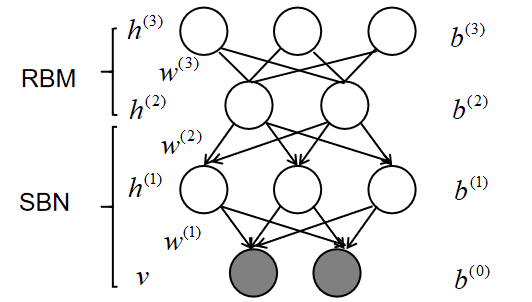
\includegraphics[width=.55\textwidth]{微信图片_20200407114236.png}
    \caption{Deep Belief Network的概率图模型}
    \label{fig:my_label_1}
\end{figure}
从上述图中,可以看出DBN是一个混合模型,上面是Restricted Boltzmann Model(RBM)模型,下面是一个Sigmoid Belief Network(SBN)。而每个节点都服从0/1的伯努利分布,实际上就是一个分层模型。深层的含义,我们将会在下文中描述。注意,这里的$w$是用来描述节点直接连接权重的矩阵。
\subsection{SBN简要回顾}
Sigmoid Belief Network的概率图模型如下所示:
\begin{figure}[H]
    \centering
    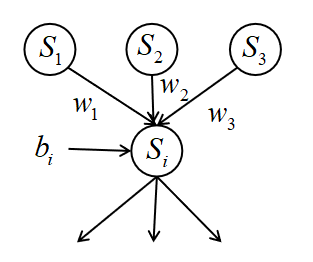
\includegraphics[width=.3\textwidth]{微信图片_20200407120853.png}
    \caption{Sigmoid Belief Network的概率图模型}
    \label{fig:my_label_1}
\end{figure}
其中,
\begin{equation}
    P(S_i=1) = \frac{1}{ 1 + \exp\{ b_i + w_1s_1 + w_2s_2 + w_3s_3 \}}
\end{equation}
\subsection{DBN的联合概率分布}
在之前的章节我们详细的描述过了,在使用极大似然估计法中基本离不开求联合概率分布。所以,这里需要求DBN的联合概率分布,而求联合概率分布最终的就是因子分解。那么,我们首先要理顺一下各层之间的依赖关系。显然,$v$层只和$h^{(1)}$有关,$h^{(1)}$层只和$h^{(2)}$,那么有:
\begin{equation}
    \begin{split}
        P(v,h^{(1)},h^{(2)},h^{(3)}) = & P(v|h^{(1)},h^{(2)},h^{(3)})P(h^{(1)},h^{(2)},h^{(3)}) \\
        = & P(v|h^{(1)})P(h^{(1)},h^{(2)},h^{(3)}) \\
        = & P(v|h^{(1)})P(h^{(1)}|h^{(2)},h^{(3)})P(h^{(2)},h^{(3)}) \\
        = & \prod_i P(v_i|h^{(1)}) \prod_j P(h^{(1)}_j|h^{(2)},h^{(3)})P(h^{(2)},h^{(3)}) \\
    \end{split}
\end{equation}
下一步则是将这三个部分分布表示。根据公式(1)的结论,可以类比的得出:
\begin{equation}
    \begin{split}
       &  P(v_i|h^{(1)}) = \text{sigmoid}\left(\left(W^{(1)}_{:,i}\right)^T \cdot h^{(1)} + b^{(0)}_i\right) \\
       &  P(h_j^{(1)}|h^{(2)}) = \text{sigmoid}\left(\left(W^{(2)}_{:,j}\right)^T \cdot h^{(2)} + b^{(1)}_j\right)
    \end{split}
\end{equation}
而$h^{(2)}$和$h^{(3)}$之间是RBM模型,沿用在RBM那一章讲的Boltzmann Distribution可以得到:
\begin{equation}
    P(h^{(2)},h^{(3)}) = \frac{1}{Z} \exp\left\{ \left(h^{(3)}\right)^Tw^{(3)}h^{(2)} + \left(h^{(2)}\right)^T b^{(2)} + \left(h^{(3)}\right)^T b^{(3)} \right\}
\end{equation}

其中参数为:
\begin{equation}
    \theta = \{ W^{(1)},W^{(2)},W^{(3)},b^{(0)},b^{(1)},b^{(2)},b^{(3)} \}
\end{equation}

\subsection{小结}
本小节,我们讲述了DBN的Representation,而很多小伙伴会疑惑为什么是一个hybrid model,为什么要一半用有向图,一般用无向图,这样做有什么好处,作者是如何思考出来的,深层含义是什么?这些问题,将在下一节进行描述。

\section{DBN叠加动机}
上一节弄清楚了DBN的model representation,这一小节主要是直觉性的介绍一个DBN的思路。为什么可以混在一起,为什么Deep Belief Network可以看成Stacking RBM。我们将从RBM引出DBN的模型。
\subsection{改进RBM的原因}
首先,我们看看原始的RBM模型的表达方式,RBM的求解在“直面配分函数”那章讲到了,是使用对比散度的方法求解。概率图模型如下图所示:
\begin{figure}[H]
    \centering
    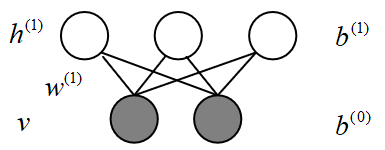
\includegraphics[width=.4\textwidth]{微信图片_20200407131510.png}
    \caption{Restricted Boltzmann Distribution的概率图模型}
    \label{fig:my_label_1}
\end{figure}
首先,回忆一下当时是如何进行求解的。通过一系列的化简,得到了log likelihood gradient的表达形式:
\begin{equation}\begin{aligned}
\frac{\partial}{\partial w_{i j}} \log P(v) &=\sum_{h} \sum_{v} P(h, v)\left(-h_{i} v_{j}\right)-\sum_{h} P(h | v)\left(-h_{i} v_{j}\right) \\
&=\sum_{h} P(h | v) h_{i} v_{j}-\sum_{h} \sum_{v} P(h, v) h_{i} v_{j}
\end{aligned}\end{equation}
但是公式(6)的计算过于复杂,基本是intractable。所以提出了用结合梯度上升法的Gibbs采样来求梯度,从而使得$P(v)$的Log Likelihood 达到最大,公式如下所示:
\begin{gather}
\Delta w_{i j} \leftarrow-\Delta w_{i j}+\frac{\partial}{\partial w_{i j}} \log P(v) \\
\frac{\partial}{\partial w_{i j}} \log P(v)=P\left(h_{i}=1 | v^{(0)}\right) v_{j}^{(0)}-P\left(h_{i}=1 | v^{(k)}\right) v_{j}^{(k)}
\end{gather}
那么,按DBN的叠加方式一定会取得更好的效果吗?结果是不用废话的。\textbf{需要明确一点,引入RBM是为了探究观测变量的数据结构的关系,其中未
观察变量被看作观察变量发生的原因。}

所以,模型的关注重点实际上是$v$,而$h$不过是我们为了探究$v$的数据结构和发生的原因,所做的模型假设而已。$v$是没有标签的数据,可以认为是RBM方法生成的,那么这个RBM有没有办法改进,让生成的数据更接近真实分布?

\subsection{RBM的改进}
根据图3可知,
\begin{equation}
    P(v) = \sum_{h^{(1)}} P(v, h^{(1)}) = \sum_{h^{(1)}} P(h^{(1)})P(v| h^{(1)})
\end{equation}
通常$P(h^{(1)})$看成是prior先验,$P(v| h^{(1)})$则看成是一个生成过程。RBM在无向图中并没有箭头,无向图可以看成是一个双向的有向图,如下所示:
\begin{figure}[H]
    \centering
    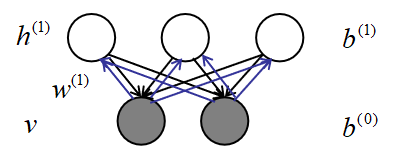
\includegraphics[width=.4\textwidth]{微信图片_20200407163930.png}
    \caption{Restricted Boltzmann Distribution的有向图概率图模型}
    \label{fig:my_label_1}
\end{figure}
这样,将无向图改写成有向图,可以把概率图分成$h\longrightarrow v$和$v\longrightarrow h$两个过程。两个过程的权重都是一样的。那么假定在RBM已经学习出来的情况下($w^{(1)}$的参数是确定的),$P(v|h^{(1)})$可以看成是$h\longrightarrow v$,显示是不变得,而$P(h^{(1)})$显然也是确定的,和$v\longrightarrow h$过程相关,$w^{(1)}$和$v$都是确定的。

由于$P(v) = \sum_{h^{(1)}} P(h^{(1)})P(v| h^{(1)})$, $P(h^{(1)})$和$P(v| h^{(1)})$都是确定的,那么$P(v)$就是确定的。那么,可以衍生出一种很自然的想法,\textbf{可不可以不用$w$来表示$P(h^{(1)})$,给$P(h^{(1)})$重新赋一组参数,create一个新的模型来对$P(h^{(1)})$重新建模,用另一个RBM来表示$P(h^{(1)})$,从而通过提高$P(h^{(1)})$的办法来提高$P(v)$。}

那么,怎么学习呢?可以添加一层RBM,这样就可以给$P(h^{(1)})$重新赋一组参数,然后通过新的RBM参数进行优化的方式来提高$P(h^{(1)})$。如下图所示:
\begin{figure}[H]
    \centering
    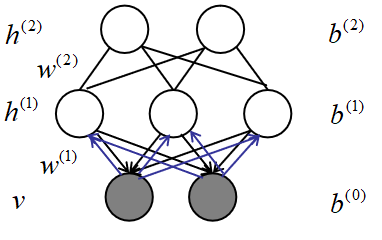
\includegraphics[width=.4\textwidth]{微信图片_20200407170000.png}
    \caption{Restricted Boltzmann Machine的改进示意图}
    \label{fig:my_label_1}
\end{figure}
由此,可以认为这样一个模型,比原来的RBM更好,因为假设$P(v|b^{(1)})$是固定的,实际可以优化$P(h^{(1)})$来进一步提高模型的性能。同样的思路,可以用同样的办法来优化$P(h^{(2)})$,所以就达到了不停的往上加的效果。

我们希望在训练$h^{(1)}$层的时候,希望$v$不会对$h^{(1)}$造成影响,否则计算复杂度就太高了。所以,就假设在训练$h^{(1)}$的过程中和$v$无关,所以概率图模型就变为:
\begin{figure}[H]
    \centering
    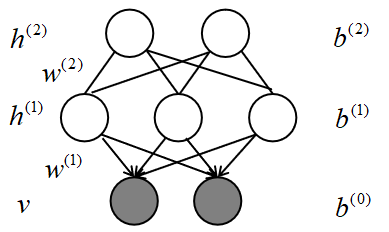
\includegraphics[width=.4\textwidth]{微信图片_20200407171216.png}
    \caption{服从假设后的RBM改进示意图}
    \label{fig:my_label_1}
\end{figure}
实际上讲解到了这里,DBN的演变模型大概都已经出来了。我觉得这个系列演变的思路在于\textbf{关于$P(h^{(1)})$和$P(v| h^{(1)})$两个部分的计算分开优化,从而发挥最大的效果,尽可能的提高模型的性能}。

\subsection{为什么DBM会更好?}
下面将给出推导来证明,为什么添加DBM会使得模型变得更好。首先计算一些RBM的下界。
\begin{equation}
    \begin{split}
        \log P(v) = & \log \sum_{h^{(1)}} P(v,h^{(1)}) \\
        = & \log \sum_{h^{(1)}} Q(h^{(1)}|v) \frac{P(v,h^{(1)})}{Q(h^{(1)}|v)} \\
        = & \log \mathbb{E}_{Q(h^{(1)}|v)} \left[ \frac{P(v,h^{(1)})}{Q(h^{(1)}|v)} \right] \\
        \geq & \mathbb{E}_{Q(h^{(1)}|v)} \log \left[ \frac{P(v,h^{(1)})}{Q(h^{(1)}|v)} \right] \ \text{(琴生不等式)} \\
        = & \sum_{h^{(1)}} Q(h^{(1)}|v) \left[ \log P(v,h^{(1)}) - \log Q(h^{(1)}|v) \right] \\
        = & \sum_{h^{(1)}} Q(h^{(1)}|v) \left[ \log P(v|h^{(1)}) + \log P(h^{(1)}) - \log Q(h^{(1)}|v) \right] \\
    \end{split}
\end{equation}
那么,$\sum_{h^{(1)}} Q(h^{(1)}|v) \left[ \log P(v|h^{(1)}) + \log P(h^{(1)}) - \log Q(h^{(1)}|v) \right]$就是原来的RBM的下界。在RBM中当整个模型训练完毕之后,$w$已经是确定的,那么$\log P(v|h^{(1)})$和$\log Q(h^{(1)}|v)$都可以看成是一个常数,而$Q(h^{(1)}|v)$是一个后验。所以下界被我们写为:
\begin{equation}
    \sum_{h^{(1)}} Q(h^{(1)}|v) \log P(h^{(1)}) + C
\end{equation}
在RBM中$P(h^{(1)})$是固定的,而在DBM中并不是固定的,而将通过优化$P(h^{(1)})$来提升模型的性能。\textbf{而$h^{(2)}$的目的就是令$h^{(1)}$的likelihood达到最大。}那么如果不加层的话,普通的RBM中公式(11)中的所有项都是确定的,而加了层之后,$P(h^{(1)})$不是确定的,而且可以被进一步优化。这样一波操作,\textbf{就相当于变相的提高了$\log P(v)$的ELBO,而下界增大以后,就等价于可以将$P(v)$的值提的更高,所以加层以后,模型的性能会更好。}
 
加层以后,$w^{(2)}$是需要赋予初始值的,那么令$w^{(2)} = {w^{(1)}}^T$。这样做的意义在于,第二层还没有学习之前性能就已经达到了不加层时的效果了。那么,可以保证加层之后的模型的性能是有下界的,大于等于原始的RBM。随着学习的进行,会提高ELBO从而获得比RBM更好的$P(v)$,模型可以得到更高的$P(v)$就意味着越接近真实分布,性能越好。

在RBM中$P(h^{(1)})$的参数是由$w^{(1)}$决定的,加层以后$P(h^{(1)})$的参数发生了改变是由$w^{(2)}$决定的。

\subsection{小结}
本节主要讲述的是DBN的思想来源,为什么DBN会产生较好的效果。DBN的主要思路就是通过单独优化先验来提升下界,从而使似然函数最大化,它分离了先验和似然的求解过程,使用两组不同的参数,分开优化,从而获得较好的效果。接下来,将描述其学习过程。

\section{贪心逐层预训练}
\subsection{近似推断的基本思想}
本节主要是以一个传统的RBM的角度来看DBN的Learning。在上一小节,已经较为详细的论述了,每加一层就会使得ELBO增加一些。假如,先只引入一个隐藏层$h^{(1)}$,那么有:
\begin{equation}
    \begin{split}
        \log P(v) \geq & \text{ELBO} \\
        = & \sum_{h^{(1)}} Q(h^{(1)}|v) \left[ \log P(v,h^{(1)}) - \log Q(h^{(1)}|v) \right] \\
        = & \sum_{h^{(1)}} Q(h^{(1)}|v) \log P(v,h^{(1)}) - H\left( \log Q(h^{(1)}|v)\right) \\
    \end{split}
\end{equation}
而$\log P(v,h^{(1)}) = \log P(v|h^{(1)}) + \log P(h^{(1)})$,通过将当层以下层的参数全部固定,然后新建一个RBM来优化$P(h^{(1)})$,从而达到优化ELBO的目的。

很多同学会好奇,这个$Q(h^{(1)}|v)$是什么?在前面的近似推断和EM算法的部分,都做了详细的描述。$Q(h^{(1)}|v)$是用来近似真实后验$P(h^{(1)}|v)$的简单分布,当且仅当$Q(h^{(1)}|v) = P(h^{(1)}|v)$时等号成立。但是为什么要近似推断呢?

虽然,在原始的RBM中,RBM的后验是可以计算的。因为在RBM的无向图模型中,可观测变量都已知的情况下,不可观测变量之间都是相互独立的,所以,RBM模型是可分解的,也意味着可降低复杂度,后验计算比较简单。

但是,在DBM中就不一样了,观察图1很容易得出,当可观测变量$v$被观测时。根据D-Separation中的Head to Head原则可得$h^{(1)}$中的节点之间都是相互联系的,这个现象也被称作Explain away现象。所以,$P(h^{(1)}|v)$是不可分解的,而且如果层数比较多的话,还要考虑对$h^{(1)}$和$h^{(2)}$求边缘分布,这个计算基本是intractable。所以,精确推断是搞不定了,需要用$Q(h^{(1)}|v)$来近似$P(h^{(1)}|v)$。

\subsection{训练方法}
现在的问题是$Q(h^{(1)}|v)$指的是一个近似分布,但是这个分布怎么求呢?注意,我们采取的逐层训练的方法,你可以理解是前馈神经网络一样,求对某层求解时,假设其他层的参数都是固定的,不予考虑,从下往上一层一层的训练。

求解的思路是这样的,假设$v$和$h^{(1)}$之间是无向图,那么这两层之间可以看成是一个RBM,因为是RBM就不存在不可分解的问题,后验计算比较方便,这时$Q(h^{(1)}|v) = P(h^{(1)}|v)$,可以得到:
\begin{equation}
    Q(h^{(1)}|v) = \prod_i Q(h^{(1)}_i|v) = \prod_i \text{sigmoid}\left( w^{(1)}_{i,:} + b^{(1)}_i \right)
\end{equation}
利用这个后验分布,可以采样得出$h^{(1)}$层的样本,然后利用同样的办法求得$h^{(2)}$层,这样一层一层的往上计算。注意到,最上面一层是一个真实的RBM了,因为把无向图变成有向图的目的就是为了在上面加一层,到了最上面一层了,不需要再往上加了,理所应当就保留了无向图结构。

\subsection{模型的优缺点}
实际上,真实的后验分布$P(h^{(1)}|v)$是计算不出来的,我们采用了假设的方法,从而近似的计算了一个分布$Q(h^{(1)}|v)$来代替后验分布$P(h^{(1)}|v)$。但是,实际上这两个分布之间的差距还是没那么小。所以,DBN一个硬伤就是它的ELBO是比较松散的(loose),那么就收敛性就不太好,收敛速率也可能比较低。

模型的优点是,从上而下进行采样比较简单,在最顶层(假设为第$t$层)的RBM的$w$和$b$都确定的情况下,通过Gibbs采样可以得到$h^{(t-1)}$层的样本,然后下面的所有层都是有向图模型,有向图模型的采样就相对很简单了,一层一层按照拓扑关系才就可以了。

\section{总结}
不得不说,老师讲的越来与抽象了,特别是涉及到思维层面的东西不太好理解。但是,确实给我的机器学习的研究生涯带来了不少启发。本章主要是介绍深度置信网络(Deep Belief Network,DBN)。首先介绍的是什么是DBN,DBN的特点和DBN的Model Representation;然后介绍了传统的RBM模型的劣势,从而提出了在RBM模型训练完毕以后,对先验进一步优化的思路来提高下界,所以需要设计一个RBM来对先验进行优化,这样就得到了DBN的雏形,同时也充分的表明了DBN在RBM基础上改进的有效性。最后,介绍了DBN的逐层固定的训练思路,并且讲述了由于概率图的不可分解性,导致后验计算的非常困难。所以用近似推断的方法来计算后验,但是由于近似分布和真实分布之间有一定的差距,导致算法的下界比较松散,收敛性能一般。但是算法的概率图基本由有向图模型构成,关系比较清晰,所以DBN算法的采样非常简单。






\end{document}
